% !TeX spellcheck = cs_CZ
%file:intro_TEO.tex
{\tikzset{external/prefix={tikz/TEO/}}
 \tikzset{external/figure name/.add={ch09_}{}}
%================================= Kapitola: Základy elektrických obvodů ===========================
\chapter{Základy elektrických obvodů}
\minitoc

  \section{Struktura elektrických ob\-vo\-dů}
    Ke každému skutečnému, fyzicky realizovanému, elektrickému obvodu lze nakreslit 
    \textbf{obvodové schéma}. Toto schéma je vlastně \emph{obvodovým modelem} skutečného obvodu. 
    Obvodový model je sestaven ze základních obvodových prvků - \textbf{dvojpólů}. Název plyne z 
    důležité topologické vlastnosti dvojpólů - mají dvě svorky \cite[s.~12]{Patocka2}.
    
    \subsection{Teorie elektromagnetického pole a elektrické obvody}
      Uspokojivý výklad všech makroskopických elektromagnetických jevů, jež probíhají v 
      nepohyblivých látkových prostředích, poskytuje Maxwellova klasická teorie elektromagnetického 
      pole. Vyšetření elektromagnetického pole (tj. určení vektorů \(\vec{E}\) a \(\vec{B}\) ve 
      všech bodech zkoumané oblasti pro každý okamžik) lze vždy provést integrací Maxwellových 
      rovnic pro dané okrajové a počáteční podmínky. Rovnice elektromagnetického pole se mohou 
      mnohdy zjednodušit, např. zanedbáním Maxwellova („posuvného“) proudu proti proudu vodivému v 
      1. Maxwellově rovnici u kvazistacionárních magnetických polí, zjednodušením geometrické 
      konfigurace apod. Přesto však řada technických úloh vede k dosti náročným matematickým 
      problémům. V některých případech však lze dosáhnout \emph{podstatného zjednodušení} řešení 
      použitím metod teorie elektrických obvodů. Teorie elektromagnetického pole tím sice nepozbývá 
      svůj základní význam pro elektrotechniku, avšak teorie elektrických obvodů umožňuje 
      efektivnější koncepci řešení některých technických úloh.
      
      Přistoupíme k vysvětlení pojmu \textbf{elektrický obvod}. Různá elektrotechnická zařízení lze 
      často považovat za systém složený z jednoduchých částí rozmanitě mezi sebou spojených, jimiž 
      mohou procházet proudy. Dále budeme předpokládat, že elektromagnetické jevy v tomto systému 
      lze vyjádřit pomocí \emph{napětí a proudů}. (Nebudeme tedy používat veličin \(\vec{E}\); 
      \(\vec{B}\); \(\vec{D}\); \(\vec{H}\), jež lokálně charakterizují elektromagnetické pole.) 
      Takový systém nazýváme \emph{reálným elektrickým obvodem}. Při studiu reálného elektrického 
      obvodu se abstrahujeme od jeho nepodstatných vlastností a omezujeme se jen na ty, jež jsou 
      pro zkoumaný jev rozhodující. Touto idealizací přecházíme k jednoduššímu systému, který 
      obecně nazýváme \emph{modelem}. Modelem může být opět reálný elektrický obvod, který zkoumáme 
      \emph{experimentálně}, zde však budeme mít na zřeteli pouze abstraktní modely, které 
      vyšetřujeme teoreticky. Tyto modely, jejichž vlastnosti budeme dále zkoumat, nazýváme 
      \emph{ideálními elektrickými obvody} anebo krátce \emph{obvody}\cite[s.~19]{Meyer1978}.
      
      Sestavení obvodu, jenž dostatečně přesně vystihuje reálný elektrický obvod v jeho provozních 
      podmínkách, není předmětem teorie obvodů, nýbrž disciplín, které teorii obvodů používají 
      (např. teorie elektrických strojů, elektroenergetiky, radiotechniky, sdělovací 
      elektrotechniky). \emph{Teorie obvodů vychází z těchto modelů a zkoumá jejich vlastnosti a 
      metody řešení}, která zpravidla mají vysoký stupeň přesnosti. Naproti tomu při sestavení 
      obvodu bychom se mohli dopustit chyby, kdybychom jej neověřovali konfrontací jeho vlastností 
      s originálem. Jelikož obvod nevyjadřuje všechny vlastnosti reálného elektrického obvodu, 
      vznikají jisté rozpory mezi teorií obvodů a Maxwellovou teorií elektromagnetického pole. 
      Například v teorii obvodů se předpokládá, že elektrická energie se přenáší vodiči obvodu — 
      lze ji snadno určit z napětí a proudů těchto vodičů. Naproti tomu z Maxwellovy teorie plyne, 
      že se veškerá energie přenáší dielektrikem v okolí vodičů; vodiče pouze určují směr toku této 
      energie. Tyto rozpory však nejsou překážkou pro používání teorie obvodů v praxi.
      
      %----------------------------------
      % image: \ref{TEO:fig_dvojpol}
      \begin{wrapfigure}{r}{5cm}
  \centering
  \begin{tikzpicture}[scale=1,>=latex']
     \filldraw[fill=green!20!white, draw=green!50!black, very thick] (-1,1) rectangle (1,0);
     \coordinate (v1) at (-2,0.5);
     \coordinate (v2) at (-1,0.5);
     \coordinate (v3) at (1,0.5);
     \coordinate (v4) at (2,0.5);
     \draw[-o] (v2) -- (v1);
     \draw[-o] (v3) -- (v4); 
  \end{tikzpicture}
  \caption{Dvojpól}
  \label{TEO:fig_dvojpol}
\end{wrapfigure}  
      %----------------------------------
      Libovolnou část obvodu, která je vyvedena k jedné dvojici svorek, nazýváme 
      \textbf{dvojpólem}; jeho schematické označení je na obr. \ref{TEO:fig_dvojpol}. Veličinu, jež 
      fyzikálně charakterizuje dvojpól, nazýváme jeho parametrem. Dvojpóly, které lze 
      charakterizovat jediným reálným parametrem, nazýváme \textbf{ideálními prvky obvodu} anebo 
      krátce \emph{prvky obvodu}.
      
      Z Maxwellovy teorie plyne, že elektromagnetické vlnění vyvolané elektromagnetickými jevy v 
      obvodu se šíří prostorem rychlostí světla. Pro jednoduchost předpokládejme, že 
      elektromagnetická vlna má harmonický průběh. Jsou-li geometrické rozměry reálného 
      elektrického obvodu zanedbatelně malé ve srovnání s délkou elektromagnetického vlnění, lze 
      rychlost jeho šíření považovat za nekonečně velkou a geometrické rozměry reálného 
      elektrického obvodu se neuplatní — napětí a proudy v tomto obvodu jsou pak pouze funkcí času 
      t. Lze jej modelovat obvodem, jehož magnetické pole je \emph{kvazistacionámi}; parametry jeho 
      dvojpólů nejsou funkcemi geometrických souřadnic. Hovoříme o \emph{obvodu se soustředěnými 
      parametry}.
      
      Nejsou-li geometrické rozměry reálného elektrického obvodu zanedbatelné vzhledem k délce 
      elektromagnetické vlny, je nutné brát v úvahu konečnou rychlost šíření elektromagnetického 
      vlnění — napětí a proudy v tomto obvodu pak budou nejen funkcemi času \(t\), ale též polohy v 
      prostoru, určené souřadnicemi \(x, y, z\) (zpravidla postačí jediná souřadnice). Parametry 
      dvojpólů takového obvodu jsou též funkcemi polohy, a proto hovoříme o \emph{obvodu s 
      rozprostřenými (rozloženými) parametry}.
            
      Teorie obvodů je úzce spjata s kybernetikou, a proto jsou některé pojmy těchto vědních oborů 
      společné. Jak známo, kybernetika se zabývá studiem \emph{systémů libovolné povahy, které jsou 
      schopny přijímat, uschovávat a zpracovávat informaci a využívat ji k řízení}. Obvod je 
      speciálním případem systému, v němž dochází k interakci s okolím na \emph{vstupu (na 
      vstupních svorkách)} a na \emph{výstupu (na výstupních svorkách)}; na vstup jsou připojeny 
      \emph{zdroje energie}, na výstup \emph{spotřebiče}. Napětí a proudy na vstupu představují 
      \emph{podněty (stimuly)} čili \emph{vstupní veličiny}, na výstupu představují \emph{odezvy 
      (reakce)} čili \emph{výstupní veličiny}.
      
      Základními vlastnostmi obvodu jsou: \emph{chování obvodu}, tj. závislost mezi podněty a 
      odezvami a \emph{struktura obvodu}, tj. vlastnosti jeho prvků a způsob jejich spojení. 
      Strukturu obvodu charakterizují jednak fyzikální vlastnosti prvků tvořících obvod, jednak 
      způsob jejich vzájemného spojení. V prvém případě hovoříme o \emph{fyzikální struktuře} 
      obvodu, ve druhém o jeho \emph{topologické (geometrické) struktuře}\cite[s.~21]{Meyer1978}.
      
      
    \subsection{Fyzikální struktura obvodů} 
      \subsubsection{Uzly a větve obvodu, orientace větví, větvové proudy a 
      napětí}\label{TEO:chap_Term}
        Místo styku dvou nebo několika svorek prvků obvodu nazýváme \emph{uzlem obvodu}. Dvojpól 
        spojující dvojici uzlů nazýváme \emph{větví obvodu}. Větve obvodu orientujeme, jestliže 
        jeden z uzlů větve zvolíme za počáteční a druhý za koncový. Větve obvodu lze orientovat 
        libovolně, avšak pro pevně zvolený časový okamžik \(t\). Protože směry proudů ve větvích se 
        mohou s časem měnit, nemusí se v obecném okamžiku \(t\) shodovat orientace větví se směry 
        proudů ve větvích. Pro obvody se soustředěnými parametry a se zavedenou orientací větví 
        definujeme: \emph{Okamžitou hodnotou větvového proudu} \(i\) budeme nazývat okamžitou 
        hodnotu proudu procházejícího průřezem větve, jehož orientace (směr normály) je dána 
        orientací větve. Z této definice plyne, že okamžitá hodnota větvového proudu je kladná v 
        čase \(t\), kdy je směr proudu ve větvi souhlasný s orientací větve a záporná pro ta \(t\), 
        kdy je směr proudu opačný. Okamžitý směr proudu budeme ve schématech vyznačovat šipkou 
        \begin{tikzpicture}\draw[-open triangle 45] (0,0) -- (1,0);\end{tikzpicture} podle obr. 
        \ref{TEO:fig_dvojpol_iu}.
        
        \begin{figure}
          \centering
          \begin{tikzpicture}[scale=1]
   \filldraw[fill=green!20!white, draw=green!50!black, very thick] (-1,1) rectangle (1,0);
   \coordinate (v1) at (-2,0.5);
   \coordinate (v2) at (-1,0.5);
   \coordinate (v3) at (1,0.5);
   \coordinate (v4) at (2,0.5);
   \draw[-o] (v2) -- (v1);
   \draw[-o] (v3) -- (v4); 
   \draw[-open triangle 45] (1.2,0.8) -- (1.8,0.8) node[right] {\(i\)};
   \draw[-triangle 45] (v1) ++ (0.2,-0.2) to [out=-45,in=-135] (1.8,0.4);
   \node[below] at (0,-0.4) {\(u\)};
\end{tikzpicture}
          \caption{Větvový proud \(i\), větvové napětí \(u\) a orientace větve}
          \label{TEO:fig_dvojpol_iu}
        \end{figure}

        \emph{Okamžitou hodnotou větvového napětí} u budeme nazývat okamžitou hodnotu napětí mezi 
        počátečním a koncovým uzlem orientované větve v daném čase \(t\). Orientaci větvového 
        napětí budeme ve schématech vyznačovat šipkou 
        \begin{tikzpicture}\draw[-triangle 45] (0,0) to (1,0);\end{tikzpicture} podle obr. 
        \ref{TEO:fig_dvojpol_iu}, přičemž šipka směřuje od počátečního ke koncovému uzlu 
        orientované dráhy, po níž se napětí měří.
        
      \subsubsection{Ideální prvky obvodu a jejich chování}
        Ideální prvky jsou z hlediska svých fyzikálních vlastností i matematického popisu 
        nejjednoduššími dvojpóly obvodu. O vodičích, které je spojují, předpokládáme, že mají 
        nulový odpor a že průchodem proudu nevzniká v jejich okolí magnetické pole. Elektrické 
        pole, jež je obecně vírové, je vně každého prvku obvodu polem potenciálním. Z toho plyne, 
        že hodnota napětí mezi dvojicemi uzlů obvodu nezávisí na tvaru integrační dráhy (tj. na 
        uspořádání přívodů voltmetru) mezi těmito uzly.
        
        Ideální prvky obvodu dělíme na aktivní a pasívní.
        
        \textbf{Aktivní prvky} jsou zdroje elektrické energie (generátory). Zpravidla přijímají 
        neelektrickou formu energie (např. mechanickou, chemickou, tepelnou) a přeměňují ji na 
        elektrickou energii, kterou dodávají do obvodu. Rozlišujeme dva typy aktivních prvků:
        \begin{itemize}
          \item ideální zdroje napětí obr. 5a), jejichž jediným parametrem je svorkové napětí     
                \(u_0 =  u_0(t)\)
          \item ideální zdroje proudu obr. 5b), jejichž jediným parametrem je dodávaný proud      
                \(i_0 = i_0(t)\)
        \end{itemize}
        
        Napětím ideálního napěťového zdroje rozumíme okamžitou hodnotu napětí mezi svorkami zdroje 
        v pořadí, jež stanovíme tím, že první svorku označíme znakem + a druhou znakem —. Svorky 
        zdroje tedy tvoří uspořádanou dvojici: svorka + se bere jako první a svorka — jako druhá. U 
        zdrojů časově proměnného napětí nemusejí znaky + a — představovat skutečnou polaritu 
        svorek; jsou to referenční znaky, jež pouze vyjadřují, že udávané napětí je měřeno od 
        svorky označené + ke svorce označené —. Skutečnou polaritu svorek vyjadřují v těch 
        okamžicích, v nichž je \(u_0(t) > 0\).
        
        V teorii obvodů se ideální zdroje dělí dále na \emph{nezávislé (autonomní)} a na 
        \emph{řízené (závislé, neautonomní)}.
        \begin{itemize}
          \item \textbf{Nezávislý ideální zdroj napětí} má svorkové napětí \(u_0 = u_0(t)\) 
                nezávislé na zatížení zdroje (tj. na výkonu dodávaném zdrojem do obvodu).
          \item \textbf{Nezávislý ideální zdroj proudu} dodává do obvodu proud \(i_0 = i_0(t)\) 
                nezávislý na zatížení zdroje.
          \item \textbf{Řízený ideální zdroj napětí, řízený napětím}, má svorkové napětí, jež je 
                funkcí napětí na některé části obvodu.
          \item \textbf{Řízený ideální zdroj napětí}, řízený proudem, má svorkové napětí, jež je 
                funkcí proudu v některé části obvodu.
          \item \textbf{Řízený ideální zdroj proudu}, řízený napětím, dodává proud, jenž je funkcí 
                napětí v některé části obvodu.
          \item \textbf{Řízený ideální zdroj proudu}, řízený proudem, dodává proud, jenž je funkcí 
                proudu v některé části obvodu.
        \end{itemize}
        
        S řízenými zdroji se často setkáváme v elektronice. Například zesilovač napětí lze nahradit 
        řízeným ideálním zdrojem napětí, přičemž napětí zdroje je funkcí napětí nebo proudu 
        přiváděného na vstup zesilovače.

        \emph{Základních obvodových prvků} je celkem pět: rezistor, cívka, kondenzátor, ideální 
        zdroj napětí, ideální zdroj proudu. Zdůrazněme následující skutečnosti:
        \begin{itemize}
          \itemsep0em 
          \item Každý ze základních prvků je uvažován jako \textbf{ideální} (nemá žádné jiné  
                parazitní vlastnosti).
          \item Kombinací základních prvků vznikne \textbf{náhradní zapojení} skutečného prvku, 
                včetně jeho parazitních vlastností.
          \item Z pěti základních prvků je tedy možno sestavit \textbf{libovolný obvodový model}
                (elektrický obvod) \textbf{pasivní} i \textbf{aktivní}.
          \item U \textbf{aktivních obvodů} (např. zesilovačů) se uplatňují řiditelné, neboli
                parametrické prvky. Typickým příkladem je bipolární tranzistor, jenž je řízen 
                proudem do báze.
        \end{itemize}
      
      \subsubsection{Přizpůsobení zdroje a spotřebiče}
        Zajímavé je sledovat, jak se mění napětí, proud a výkon na spotřebiči v závislosti na 
        poměru odporu spotřebiče a vnitřního odporu zdroje. Jednoduchou úvahou lze usoudit, že 
        největší napětí je naprázdno při nekonečném odporu spotřebiče a největší proud bude při 
        nulovém odporu spotřebiče (zkratu). Maximum výkonu nebude ani při maximálním proudu, 
        protože napětí na zkratu je nulové, ani při maximálním napětí, protože obvodem neprotéká 
        proud. Výkon, který je součinem napětí a proudu, je v obou případech nulový.
        
        Pokud připojíme k náhradnímu napěťovému schématu zdroje spotřebič, bude pro protékající 
        proud platit: \(I = \frac{U_i}{R_i + R_z}\). Po dosazení vztahu pro napětí na spotřebiči, 
        které je shodné se svorkovým napětím zdroje \(U=I\cdot R_z\), získáme vztah: \(U = 
        U_i\frac{R_z}{R_i + R_z}\).
        
  \section{Topologická struktura obvodů}
    Topologické vlastnosti obvodů lze studovat pomocí teorie grafů, jež je odvětvím 
    topologie\footnote{Topologie je moderní	matematická disciplína zabývající se studiem takových 
    vlastností objektů, jež jsou invariantní vzhledem k vzájemně jednoznačnému spojitému zobrazení, 
    jehož inverzní zobrazení je též spojité. Tyto vlastnosti se nazývají topologické vlastnosti 
    (topologické invarianty). (Zmíněné zobrazení lze názorně interpretovat jako takové deformování 
    zkoumaného objektu, při němž se nesmí objekt porušit ani spojovat.) Například hovoříme-li o 
    topologických vlastnostech obvodů, nemáme na mysli způsob rozmístění prvků obvodu v prostoru, 
    nýbrž počet prvků a vlastnosti jejich vzájemného spojení. Studium topologických vlastností 
    obvodů spadá do odvětví topologie, zvaného teorie grafů. Základy teorie grafů byly vybudovány 
    právě na základě potřeb teorie obvodů (G. Kirchhoff).}
    
    \subsection{Základní pojmy z topologie obvodů}
      Definice grafu obvodu. Mějme v prostoru body \(B_1; B_2;\cdots; B_{n_u}\) — nazveme je uzly. 
      Dvojice těchto uzlů nechť tvoří krajní body navzájem se neprotínajících oblouků (tzv. 
      topologických úseček) \(v_1; v_2; \cdots; v_{n_v}\) — nazveme je \emph{větvemi}. Množinu 
      všech větví pak nazýváme \emph{grafem obvodu}.
      
      Graf obvodu tedy vyjadřuje topologickou strukturu obvodu a získáme jej tím, že jej 
      abstrahujeme od fyzikálních vlastností prvků obvodu. U grafu nás nezajímají jeho metrické 
      vlastnosti, tj. uzly grafu lze libovolně rozmístit a jeho větve lze libovolně deformovat, 
      avšak nesmíme je přerušit a po jejich deformaci je popřípadě opět spojit.
      
      Graf, který vznikne z grafu \(\mathscr{G}\) těmito úpravami, nazýváme \emph{izomorfním} (čili 
      \emph{topologicky ekvivalentním}) s grafem \(\mathscr{G}\). Na obr. \ref{TEO:fig_topo01} je 
      příklad obvodu a jeho tří izomorfních grafů.
      
      \begin{figure}[ht!]
        \centering
        \includegraphics[width=0.9\linewidth]{TEO_topo01.jpg}
        \caption{ Obvod (a) a jeho topologicky ekvivalentní (izomorfní) grafy (b), (c), (d) 
                  \cite[s.~39]{Meyer1978}}
        \label{TEO:fig_topo01}
      \end{figure}
      
      Uzly grafu jsou charakterizovány svým stupněm: \emph{stupeň uzlu} \(\varepsilon\) udává počet 
      větví grafu, jež s uvažovaným uzlem \emph{incidují}\footnote{Dva geometrické útvary nazýváme 
      \textbf{incidentní} (resp. říkáme, že spolu incidují), jestliže jeden z nich obsahuje útvar 
      druhý. Například všechny přímky procházející daným bodem jsou s ním incidentní, nebo všechny 
      křivky ležící na ploše s ní incidují.}. Uzel stupně \(0\) (tzv. \emph{izolovaný uzel}) a uzel 
      stupně \(1\) (větev s ním incidující se nazývá \emph{izolovaná}) mají význam v matematické 
      teorii grafů, ale v grafech obvodů se setkáváme jen s uzly stupně \(\varepsilon\geqq 2\). 
      Někdy je výhodné vypustit uzly stupně \(2\) (tzv. vnitřní uzly větví) a uvažovat jen uzly 
      stupně \(\varepsilon\geqq 3\). Tím zmenšíme počet větví obvodu, avšak v jeho větvích obecně 
      nebude již jediný prvek, ale složitější dvojpól — sériové spojení prvků; např. v grafu obvodu 
      na obr. \ref{TEO:fig_topo01} jsou uzly \(B_1; B_2; B_3; B_4\) vesměs 3. stupně, uzly \(B_5; 
      B_6\) jsou 2. stupně vnitřní uzly); graf má \(n_v = 8\) větví. Omezíme-li se na uzly stupně 
      \(\varepsilon\geqq 3\), představují větve \(v_3; v4\) jedinou větev s krajními uzly \(B_2; 
      B_3\) a podobně větve \(v_7; v_6\) tvoří jedinou větev s uzly \(B_2; B_4\) graf má pak jen 
      \(n_v = 6\) větví.
      
      Dvojici grafů, jejichž izomorfismus je porušován jen uzly 2. stupně, nazýváme 
      \emph{homeomorfními}. Homeomorfní grafy jsou tedy takové grafy, jež se po odstraněni 
      některých uzlů 2. stupně stanou izomorfními.
  
  \section{Kirchhoffovy zákony}
    V této kapitole budeme formulovat Kirchhoffovy zákony a ukážeme, jak lze jejich použitím popsat 
    chováni obvodu soustavou rovnic.
    
    \subsection{Formulace prvního a druhého Kirchhoffova zákona}
      Kirchhoffovy zákony, spolu se vztahy mezi napětími a proudy pasivních prvků (tab. 3), mají 
      pro teorii obvodů základní význam. \emph{Platí pro jakýkoliv obvod se soustředěnými 
      parametry}, lineární i nelineární, s parametry časově konstantními i s časově proměnnými. Z 
      hlediska teorie obvodů lze Kirchhoffovy zákony považovat za postuláty, z nichž tato teorie 
      vychází. Z hlediska teorie elektromagnetického pole jsou však důsledkem plynoucím z 
      Maxwellovy teorie.
      
%     \begin{mdframed}[style=MyFrame]
      \textbf{První Kirchhoffův zákon}. Pro libovolný uzel obvodu platí: Součet okamžitých hodnot 
      proudů vystupujících z uzlu a proudů vstupujících do uzlu je roven nule. Přitom proudy 
      vystupující z uzlu bereme jako kladné a proudy vstupující do uzlu jako záporné.
%     \end{mdframed} 
      
      \begin{proof}
        Uvažujme libovolný uzel obvodu \(B_j\). Obklopíme jej libovolnou uzavřenou orientovanou 
        plochou \(S\) obr. \ref{TEO:fig_KZ01}a). Vzhledem k tomu, že magnetické pole obvodu se 
        soustředěnými parametry je kvazistacionární, má rovnice kontinuity tvar
        \begin{equation}
          \oint_s \vec{J}(t)\dd{\vec{S}} = 0
        \end{equation}
        \begin{figure}[ht!]
          \centering
          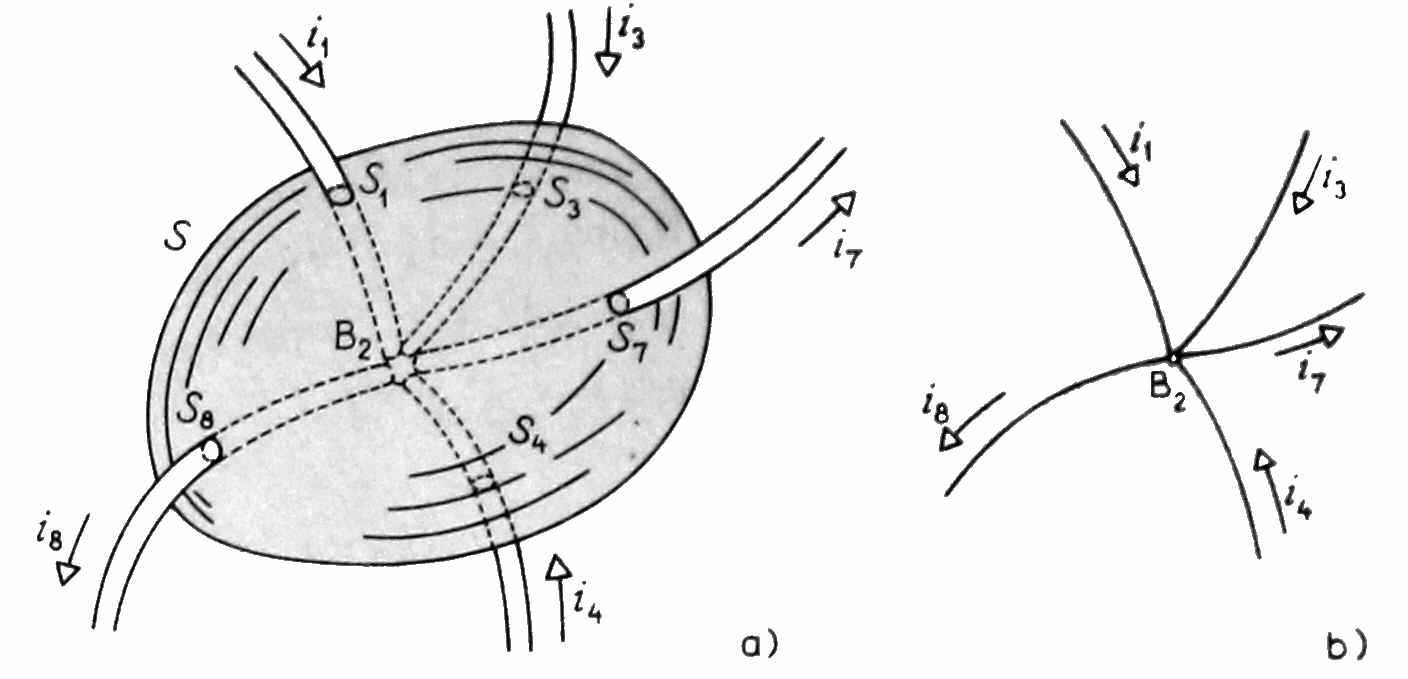
\includegraphics[width=0.9\linewidth]{TEO_KZ01.jpg}
          \caption{Uzel incidující s pěti větvemi: reálný elektrický obvod (a) a ideální obvod (b). 
                   (K odvozeni prvního Kirchhoffova zákona) \cite[s.~47]{Meyer1978}}
          \label{TEO:fig_KZ01}
        \end{figure}      
        Pro tok vektoru proudové hustoty uzavřenou plochou \(S\) podle obr. \ref{TEO:fig_KZ01}a) 
        platí
        \begin{equation}
          \oint_s \vec{J}(t)\dd{\vec{S}} = \sum_{\mathclap{\substack{k\\B_j\in v_k}}}
                                           \int_{S_k} \vec{J}(t)\dd{\vec{S}} 
        \end{equation}
        kde sumace na pravé straně rovnice je provedena přes indexy všech větví incidujících s 
        uzlem \(B_j\). Jednotliví sčítanci představují proudy vystupující z uzlu, resp. vstupující 
        do uzlu. Porovnáním obou uvedených vztahů plyne dokazovaný první Kirchhoffův zákon.
      \end{proof}
      
      Matematicky lze zapsat první Kirchhoffův zákon pro libovolný uzel obvodu \(B_j\) pomocí 
      větvových proudů \(i_k\) libovolně orientovaných větví \(v_k\)\footnote{Orientace větví 
      obvodu je libovolná, ale pevně zvolená (nezávislá na čase), viz kap. \ref{TEO:chap_Term}.} ve 
      tvaru 
      \cite[s.~47]{Meyer1978}
      \begin{equation}\label{TEO:eq_KZI}
        \sum_{\mathclap{\substack{k\\B_j\in v_k}}} \pm i_k = 0; \qquad j = 1;\ldots; n_u 
      \end{equation}
      Znaménko \(+\) platí, je-li větev \(v_k\) orientována tak, že uzel \(B_j\) je jejím 
      počátečním uzlem a znaménko \(—\) platí v opačném případě; sčítáme pro všechna \(k\), pro něž 
      uzel \(B_j\) inciduje s větví \(v_k (B_j\in v_k)\); \(n_u\) je počet všech uzlů obvodu. 
      Poznamenejme, že podle definice větvového proudu (viz kap. \ref{TEO:chap_Term}) je \(i_k > 
      0\), souhlasí-li směr proudu s orientaci větve a \(i_k < 0\) v opačném případě.
      
      Například pro uzel \(B_2\) podle obr. \ref{TEO:fig_KZ01}b) má první Kirchhoffův zákon tvar
      \begin{equation*}
        -i_1 - i_3 - i_4 + i_7 + i_8 = 0
      \end{equation*}
      Rovnice (\ref{TEO:eq_KZI}) je symbolickým zápisem prvního Kirchhoffova zákona, vyžadujícím 
      slovní komentář o tom, kdy máme brát znaménko \(+\) , kdy znaménko \(—\) a jakých hodnot 
      nabývá sčítací index \(k\). Tento zápis prvního Kirchhoffova zákona je velmi dobře použitelný 
      pro řešení jednodušších obvodů. Naproti tomu při řešení obvodů na počítači je třeba vyjádřit 
      první Kirchhoffův zákon výstižnějším zápisem ve tvaru
      \begin{equation}\label{TEO:eq_KZI_01}
        \sum\limits_{k=1}^{n_v} a_{jk} i_k = 0; \qquad j = 1;\ldots; n_u 
      \end{equation}
      \begin{figure}[ht!]
        \centering
        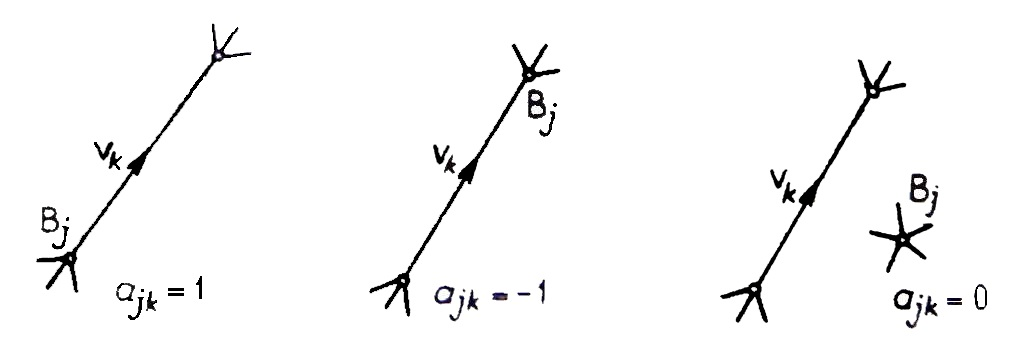
\includegraphics[width=0.9\linewidth]{TEO_KZ02.jpg}
        \caption{K určení hodnot koeficientů \(a_{jk}\) \cite[s.~47]{Meyer1978}}
        \label{TEO:fig_KZ02}
      \end{figure}
      kde koeficienty \(a_{jk}\) vyjadřují incidenci uzlů a větví v orientovaném grafu obvodu a 
      nabývají těchto hodnot: \(a_{jk} = 1\), když j-tý uzel je počátečním uzlem k-té větve, 
      \(a_{jk} = — 1\), když j-tý uzel je koncovým uzlem k-té větve a \(a_{jk} = 0\), když j-tý 
      uzel neinciduje s k-tou větví (obr. \ref{TEO:fig_KZ02}). Znaménko větvového proudu \(i_k\) 
      plyne ze souhlasnosti, resp. nesouhlasnosti orientace větve a směru větvového proudu (\(i_k > 
      0\), resp. \(i_k < 0\)).
      
      \textbf{Druhý Kirchhoffů v zákon}. Pro libovolnou orientovanou smyčku obvodu platí: Součet 
      okamžitých hodnot napětí na všech větvích incidujících s orientovanou smyčkou obvodu je roven 
      nule. Přitom napětí větví bereme jako kladná, jestliže proud ve větvi v daném okamžiku 
      prochází ve smyslu orientace smyčky a jako záporná, jestliže prochází v opačném směru.
      
      \begin{proof}
        Uvažujme libovolnou orientovanou uzavřenou křivku \(s_j\) procházející všemi uzly smyčky 
        obvodu a vedenou vně prvků (např. křivku vyznačenou na obr. \ref{TEO:fig_KZ03} tečkovaní). 
        Z vlastností ideálních prvků obvodu plyne, že II. Maxwellova rovnice v integrálním tvaru má 
        pro křivku \(s_j\) tvar
        \begin{align}
          \oint\vec{E}\dd{\vec{l}} &= 0    \label{TEO:eq_KZ01} \\
          \shortintertext{Pro oběhové napětí po křivce \(s_j\) (obr. \ref{TEO:fig_KZ03}) zároveň 
                          platí vztah}
          \oint\vec{E}\dd{\vec{l}} &= \sum_{\mathclap{\substack{k\\v_k\in s_j}}}\vec{E}\dd{\vec{l}}
        \end{align}
        Porovnáním obou uvedených vztahů plyne dokazovaný druhý Kirchhoffův zákon.
        \begin{figure}[ht!]
          \centering
          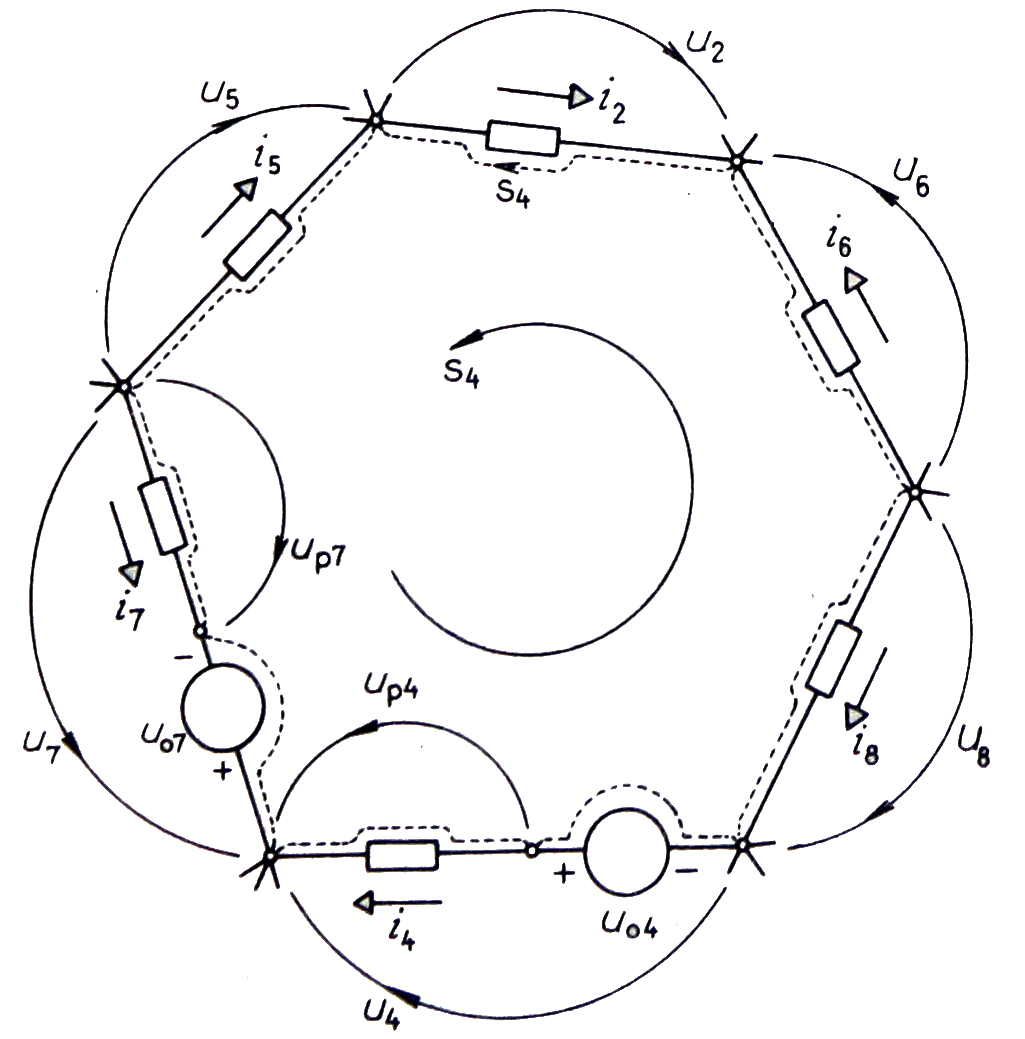
\includegraphics[width=0.7\linewidth]{TEO_KZ03.jpg}
          \caption{Smyčka incidující se šesti větvemi (K odvození druhého Kirchhoffova 
                   zákona)\cite[s.~48]{Meyer1978}}
          \label{TEO:fig_KZ03}
        \end{figure}
      \end{proof}
      Matematicky lze vyjádřit druhý Kirchhoffův zákon pro libovolnou orientovanou smyčku \(s_j\) 
      pomocí větvových napětí \(u_k\) libovolně orientovaných větví \(v_k\) ve tvaru
      \begin{equation}\label{TEO:eq_KZ03}
        \sum_{\mathclap{\substack{k\\v_k\in s_j}}} \pm u_k = 0 \qquad j=1;\cdots; n_s
      \end{equation}
      Znaménko \(+\) platí, je-li větev \(v_k\) orientována souhlasně se smyčkou \(s_j\) a znaménko 
      \(—\) platí v opačném případě; sčítáme pro všechna \(k\), pro něž větev \(v_k\) inciduje se 
      smyčkou \(s_j (v_k\in s_j)\); \(n_s\) je počet všech smyček obvodu.
      
      Například pro smyčku \(s_4\) podle obr. \ref{TEO:fig_KZ03} má druhý Kirchhoffův zákon tvar
      \begin{equation*}
        -u_2 -u_4 -u_5 +u_6 +u_7 -u_8 = 0
      \end{equation*}
      
      Vyjádření druhého Kirchhoffova zákona rovnicí (\ref{TEO:eq_KZ03}) je — obdobně jako vyjádření 
      prvního Kirchhoffova zákona rovnicí (\ref{TEO:eq_KZI}) — jen symbolickým zápisem, k němuž 
      bylo nutno připojit slovní komentář. Pro řešení obvodů na počítači je třeba vyjádřit druhý 
      Kirchhoffův zákon matematicky výstižnějším zápisem
      \begin{equation}\label{TEO:eq_KZ04}
        \sum\limits_{k=1}^{n_v} b_{jk} u_k = 0 \qquad j=1;\cdots; n_s
      \end{equation}      
      \begin{figure}[ht!]
        \centering
        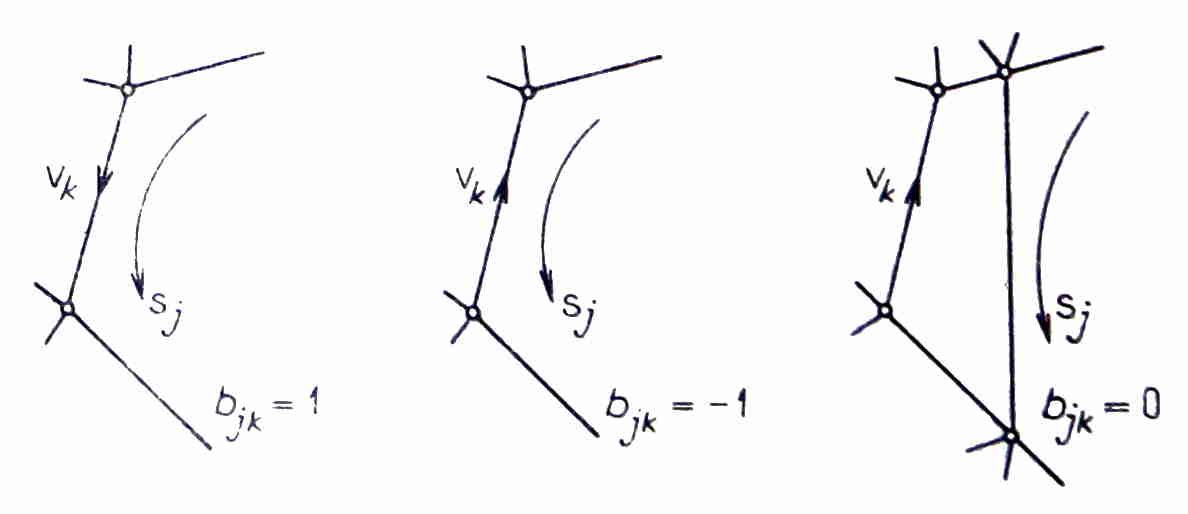
\includegraphics[width=0.9\linewidth]{TEO_KZ04.jpg}
        \caption{K určení koeficientů \(b_{jk}\) \cite[s.~49]{Meyer1978}}
        \label{TEO:fig_KZ04}
      \end{figure}      
      kde koeficienty \(b_{jk}\) vyjadřují incidenci smyček a větví v orientovaném grafu obvodu a 
      nabývají těchto hodnot: \(b_{jk} = 1\), když \(k\)-tá větev inciduje s \(j\)-tou smyčkou a 
      orientace obou se shodují, \(b_{jk} = — 1\), když \(k\)-tá větev inciduje s \(j\)-tou smyčkou 
      a orientace obou je opačná, a \(b_{jk} = 0\), když \(k\)-tá větev neinciduje s \(j\)-tou 
      smyčkou (obr. \ref{TEO:fig_KZ04}).
      
  \section{Analýza elektrických obvodů}
    Pojem \textbf{analýza} není v teorii elektrických obvodů používán v původním širokém smyslu. 
    Zejména v souvislosti s počítačovým řešením obvodů se pod analýzou obvykle rozumí 
    \emph{konkrétní metody získávání elektrických charakteristik obvodů z jejich modelů} (například 
    kmitočtová nebo stejnosměrná analýza).
    
    \subsection{Modelování, analýza, simulace}
      \emph{Analýzu} provádíme ve snaze získat informace o určitých vlastnostech zkoumaného obvodu, 
      které nás zajímají. Z praktických důvodů však zpravidla analýze nepodrobujeme samotný obvod, 
      nýbrž jeho \emph{model}. Jedním z dobrých důvodů může být skutečnost, že daný obvod dosud 
      existuje pouze v představě návrháře a před jeho výrobou je vhodné ověřit, zda je navržen 
      správně. K modelování obvodu máme k dispozici elementární modely elektrických prvků (pasivní 
      R, L, C, tranzistory, operační zesilovače apod.) ve formě matematického popisu jejich 
      fungování a  jejich elektrotechnických značek, které jsou začleněny do schématu celkového 
      zapojení. Z hlediska matematického je model obvodu představován soustavou rovnic, které lze 
      odvodit na základě rovnic dílčích elektrických prvků a Kirchhoffových rovnic, které 
      reprezentují způsob propojení součástek \cite[s.~16]{Biolek}.
      
      Při modelování obvodu je důležité nejprve uvážit, s jak složitým modelem bude vhodné 
      pracovat. Složité modely obvykle umožňují věrnější popis chování skutečného obvodu, avšak 
      současně prudce rostou požadavky na výkon analyzačního nástroje. Je zřejmé, že výpočty, které 
      provádíme jen pomocí papíru a tužky, případně kalkulačky, jsou vhodné pro analýzu méně 
      rozsáhlých obvodů s jednoduchými modely, kde nám jde buď o ověření správnosti základního 
      principu fungování, nebo o odhady chování obvodu s odhlédnutím od různých parazitních jevů a 
      vlivů reálných vlastností součástek na vlastnosti obvodu. Složité modely si můžeme dovolit 
      používat při analýze s využitím speciálních počítačových programů.

      Klasická teorie obvodů dává odpověď na otázku, s jakým minimálním počtem typů elementárních 
      modelů obvodových prvků je možné sestavit model jakkoliv složitého analogového obvodu se 
      soustředěnými parametry: jsou to pasivní prvky typu R,L,C a zdroje klasické a řízené. 
      Příslušné charakteristiky těchto prvků jsou popsány jednoduchými nebo složitými rovnicemi. Z 
      tohoto pohledu můžeme říci, že k sestavování modelů daných obvodů a k jejich využívání nemáme 
      k dispozici nic jiného než omezený počet modelů elementárních prvků s příslušnými 
      matematickými vzorci \cite[s.~17]{Biolek}.
      
      Od jisté úrovně modelování, která zajišťuje uspokojivou shodu chování modelu a originálu, je 
      možné model využívat k simulaci skutečného chování obvodu za konkrétních podmínek. Příkladem 
      může být sledování vlivu teploty na nastavený stejnosměrný pracovní bod tranzistorového 
      zesilovače. Dostáváme se k poslednímu pojmu z trojlístku \emph{modelování - analýza - 
      simulace}. Simulace je tedy něco více než analýza (v úzkém pojetí) a analýza je důležitá 
      součást simulace.
      
      \begin{figure}[ht!]
        \centering
        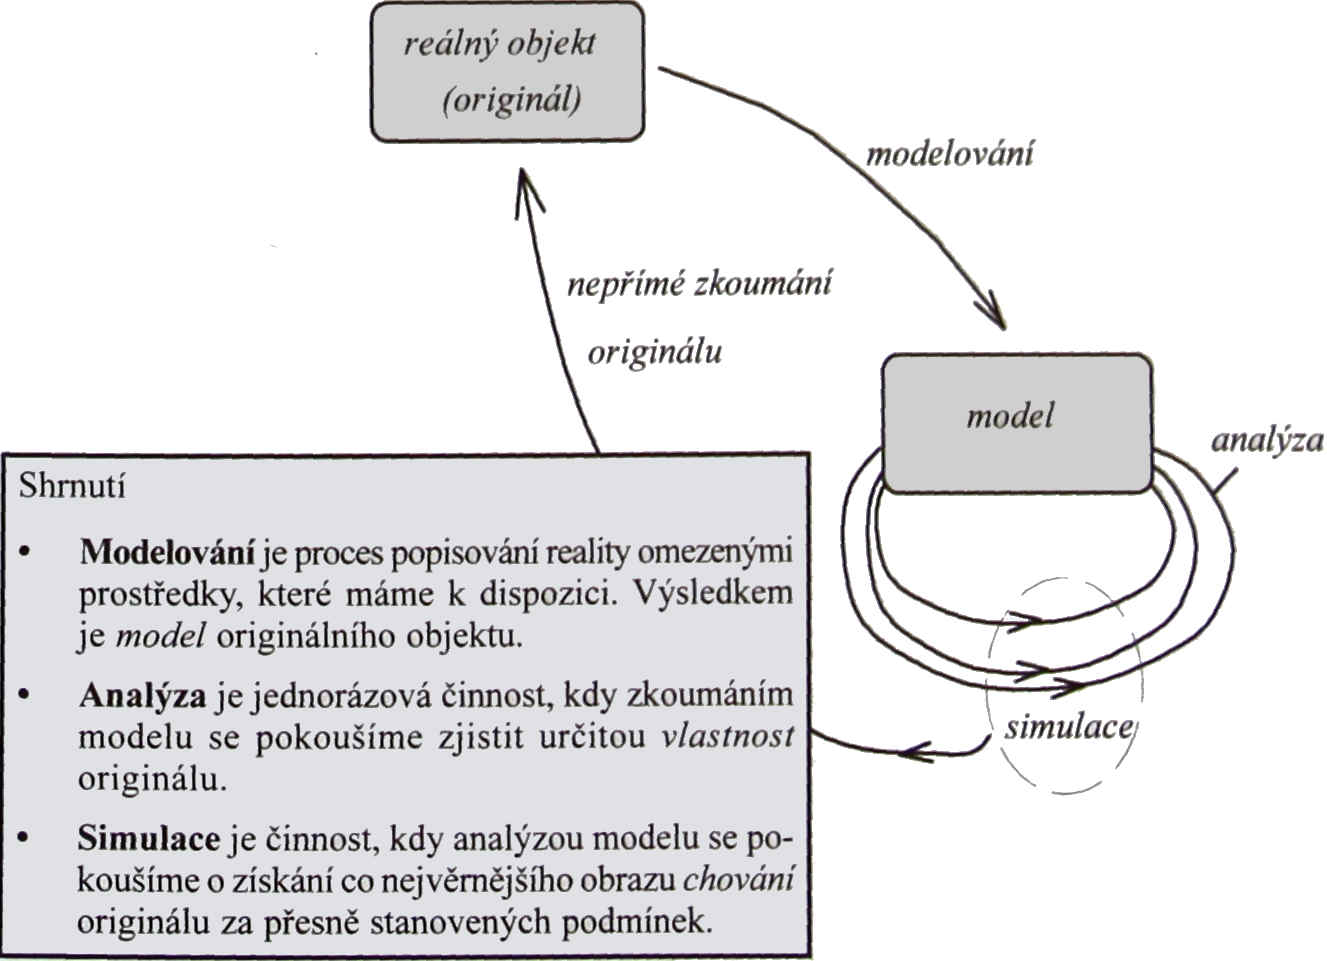
\includegraphics[width=0.95\linewidth]{Biolek_Modelovani.jpg}
        \caption{Modelováni, analýza, simulace \cite[s.~17]{Biolek}}
        \label{TEO:fig_modelovani}
      \end{figure}
      
      Shrnutí:
      \begin{itemize}
        \itemsep0em
        \item \emph{Při řešení obvodu pomocí „papíru, tužky a kalkulačky“} nejprve sestavíme model 
              obvodu ve formě schématu zapojení včetně parametrů, resp. charakteristik jednotlivých 
              součástek. Z tohoto modelu pak vzniká model matematický ve formě rovnic, které 
              vyplývají z vzájemného propojení a vlastností součástek, Kirchhoffových zákonů a 
              Ohmová zákona. Tento model pak podrobíme numerické analýze.      
        \item \emph{Při řešení pomocí počítačového programu} opět sestavujeme model obvodu,  
              většinou pomocí schematického editoru. Program je však schopen při tomto sestavování 
              účinně pomáhat tím, že je zdrojem složitých interních modelů součástek (tranzistory, 
              operační zesilovače, integrované obvody...). Vlastní sestavení rovnic, jejich řešení 
              a vizualizace výsledků je již plně v režii programu \cite[s.~18]{Biolek}.
      \end{itemize}
      
    \subsection{Metody analýzy heuristické a algoritmické}
      Metodu analýzy můžeme chápat jako konkrétní postup od modelu obvodu až po získání cíle analýzy.
      
      Všechny existující metody analýzy můžeme rozdělit na \emph{nealgoritmické (heuristické)} a 
      \emph{algoritmické}. Do první kategorie patří postupy, které řešitel volí na základě svých 
      předchozích zkušeností s využíváním tvůrčího přístupu. Například při výpočtu napětí na 
      výstupu zatíženého děliče napětí je možno nejprve sloučením zatěžovacího a pracovního 
      rezistoru převést řešení na problém děliče nezatíženého, posléze vypočítat proud děličem a 
      následně výstupní napětí. Jiným možným postupem je využití Théveninovy věty apod. 
      Algoritmická metoda oproti tomu definuje přesný postup — algoritmus, který vždy vede k cíli. 
      Výše uvedená úloha zatíženého děliče může být řešena například algoritmickou metodou 
      smyčkových proudů.
      
      Zjednodušené řečeno, heuristické metody jsou vhodné k ručnímu řešení méně rozsáhlých obvodů, 
      pokud jsme zběhlejší v elektrotechnických výpočtech a nechybí nám schopnost hledání vlastních 
      cest k cíli.
      
      Při analýze obvodů bez počítačové podpory bychom měli upřednostňovat nealgoritmické metody. 
      Pouze tam, kde je vyjadřování napěťových a proudových poměrů komplikované, např. v důsledku 
      působení speciálních obvodových prvků, je často rozumné úlohu vyřešit \emph{modifikovanou 
      metodou uzlových napětí} (část \ref{TEO:chap_MMUN}) nebo \emph{Masonovým-Coatesovým grafem} 
      (část 2.4). Každá z metod má svůj význam: nealgoritmická nutí k fyzikálnímu myšlení a k 
      pochopení funkce obvodu, který analyzujeme, algoritmická pak poskytuje účinný nástroj k 
      praktickému řešení.

  \section{Metody analýzy elektrických ob\-vo\-dů}
    \subsection{Klasická metoda uzlových napětí (MUN)}
      Metoda uzlových napětí je založena na tomto postupu:
      \begin{itemize}
       \item Jeden z uzlů obvodu se prohlásí za tzv. \textbf{referenční uzel}. Přiřadí se mu 
             číslo 0, případně v počítačovém simulátoru značka uzemnění. Vzhledem k tomuto uzlu se 
             budou vztahovat napětí ostatních uzlů obvodu. Tato napětí se nazývají \textbf{uzlová 
             napětí} a tvoří \textbf{soustavu neznámých obvodových veličin} metody. Je vhodné 
             orientovat všechna uzlová napětí tak, aby čítací šipky směřovaly do referenčního uzlu. 
             Uzlová napětí jsou neznámými metody i tehdy, je-li našim konečným cílem počítat 
             jiné obvodové veličiny. Každé napětí a každý proud v obvodu jsou totiž vyjádřitelné 
             jako lineární kombinace uzlových napětí.
       \item Pro každý uzel obvodu, vyjma referenčního, sestavíme rovnici 1. KZ ve tvaru:
             \emph{součet proudů tekoucích dovnitř uzlu z vnějších zdrojů proudu  = součtu proudů
             vytékajících větvemi obvodu ven z uzlu.}
       \item Rovnice vyřešíme, tj. získáme velikosti uzlových napětí. Z nich pak dopočteme  
             požadovaný výsledek analýzy.
      \end{itemize}
      
      Metodu uzlových napětí lze objasnit na příkladu zapojení na obr. \ref{TEO:fig_MMUN03}. Je
      třeba určit proud $I_{x2}$ 
      %----------------------------------
      % \ref{TEO:fig_MMUN03}; Biolek_MUN_priklad.pdf
        %\documentclass{article}
%  \usepackage{fontspec,xltxtra,xunicode,unicode-math} 
%  \usepackage{siunitx}
%  \usepackage{tikz}
%    \usetikzlibrary{intersections}
%    \usetikzlibrary{calc}
%    \usetikzlibrary{positioning}
%    \usetikzlibrary{arrows}
%    \tikzstyle{every node}=[font=\small]
%    \tikzstyle{every path}=[line width=0.8pt,line cap=round,line join=round]
%  \usepackage[american, 
%              europeanresistor, cuteinductors, smartlabels]{circuitikz}
%    \ctikzset{bipoles/thickness=1}
%    \ctikzset{bipoles/length=0.8cm}
  
% \begin{document}
  \begin{figure}[htp]
    \centering
\begin{circuitikz}[scale=2, every node/.style={font=\footnotesize}, european voltages]
  \node (0,0) (B) {};
  \node [left =2.5cm of B](A) {};
  \node [right=2.5cm of B](C) {};
  \node [below=2.5cm of B](D) {};
  \node [below=2.5cm of A](E) {};
  \node [below=2.5cm of C](F) {};
  \node [above=1cm of A](G) {};
  \node [above=1cm of C](H) {};

  \ctikzset{current/distance = .5}
  \ctikzset{bipoles/resistor/voltage/distance from node/.initial = .5}
  \draw[red, line width=2pt] (F)
    to[short, color =red, i>_= $i_x$](C);
  \draw (A) 
    to[R ,l=$\substack{\displaystyle\hfill R_2\\\displaystyle \SI{2}{\kohm}}$,%
        v_>=$\substack{\phantom{a}\\\displaystyle U_1-U_2}$, i>^= $i_2$, *-*] (B) node[above] {$2$}
    to[R, l=$\substack{\displaystyle\hfill R_3 \\\displaystyle \SI{2}{\kohm}}$,%
        v_>=$\substack{\phantom{a}\\\displaystyle U_2}$, i^>= $i_3$, *-*] (C);
  \draw (B) 
    to[R, l_=$\substack{\displaystyle\hfill R_4 \\ \displaystyle\SI{2}{\kohm}}$,%
         i>_=$i_4$,-*] (D); 
  \draw (A) 
    to[R, l_=$\substack{\displaystyle\hfill R_1 \\\displaystyle \SI{6}{\kohm}}$,%
         i>_=$i_1$] (E) 
    to[short](D) node[below, red] {$0$};
  \draw (C) 
    to[short] (H) 
    to[I, i^=$\SI{1}{\milli\ampere}$] (G) 
    to[short] (A) node[left] {$1$};
  \ctikzset{voltage/distance from node=0.5}
  \draw (D.north) 
    to [open, v^=$U_1$] (A.north);
  \draw (F.north) 
    to [open, v^=$U_2$](B.north);
  \draw[red, line width=2pt] (D) 
    to[short, color =red, *-] (D -| C);
\end{circuitikz}
    \caption{Řešení obvodu metodu uzlových napětí - MUN \cite[s.~62]{Biolek}}
    \label{TEO:fig_MMUN03}
  \end{figure}
% \end{document}  
      %----------------------------------       
      Nejprve očíslujeme uzly. Zvolíme referenční uzel a přiřadíme mu číslo 0. Zde je třeba  
      zdůraznit, že referenční uzel je možno volit zcela libovolně. Většinou se volí tak, aby 
      případné hledané napětí bylo rovno jednomu z napětí uzlových. Dále si všimneme, že uzel, v 
      němž je se spojuje rezistor $R_3$ a proudový zdroj, je vlastně součástí referenčního uzlu a 
      jako takový se přídavně nečísluje - má již označení 0.
      
      Vyznačená uzlová napětí $U_1$ a $U_2$ tvoří soustavu dvou neznámých, k níž musíme sestavit 
      dvě rovnice. Budou to rovnice 1. KZ pro uzly 1 a 2. Protože počítáme proud $I_{x2}$, postačí 
      určit uzlové napětí $U_2$. Z něj totiž snadno určíme proud rezistorem $R_3$ a z něj $I_{x2}$.
      
      Podle obr. \ref{TEO:fig_MMUN03} napíšeme 1. KZ pro rovnováhu proudů v uzlech 1 a 2:
      \begin{align*}
        \text{uzel 1:} \qquad I &=  I_{R1} + I_{R2}            \\
        \text{uzel 2:} \qquad 0 &= -I_{R1} + I_{R2} + I_{R4}  
      \end{align*}
      
      Orientaci čítacích šipek větvových proudů můžeme volit naprosto libovolně. Pokud se v 
      orientaci zmýlíme, vyjde u daného proudu opačné znaménko.
      
      Větvové proudy na pravé straně rovnic vyjádříme pomocí větvových vodivostí a větvových 
      napětí, která závisí na uzlových napětí (viz obr. \ref{TEO:fig_MMUN03}):
      \begin{align}
       \text{uzel 1:} \qquad I &=  G_1U_1 + G_2(U_1-U_2)             \nonumber              \\ 
       \text{uzel 2:} \qquad 0 &= -G_2(U_1-U_2) + G_3U_2 + G_4U_2    \nonumber              \\
       \shortintertext{Vytknutím neznámých upravíme rovnice na konečný tvar}
       \text{uzel 1:} \qquad I &=  (G_1 + G_2)U_1 - G_2U_2           \label{TEO:eq_MUN_pr}  \\ 
       \text{uzel 2:} \qquad 0 &= -G_2U_1 + (G_2 + G_3 + G_4)U_2     \nonumber
       \shortintertext{Dosadíme-li vodivosti v [mS], vyjdou proudy na levé straně v [mA]}
       \text{uzel 1:} \qquad 1 &=  \frac{2}{3}U_1 - \frac{1}{2}U_2   \nonumber              \\ 
       \text{uzel 2:} \qquad 0 &= -\frac{1}{2}U_1 + \frac{3}{2}U_2   \nonumber
       \shortintertext{Tyto rovnice dávají řešení}
                   [U_1, U_2]  &= \left[2, \frac{2}{3}\right] \text{V}  \label{TEO:eq_MUN_vysl}
      \end{align}
      Pohledem na schéma \ref{TEO:fig_MMUN03} zjistíme, že při $U_2 = \frac{2}{3}V$ bude proud 
      $I_{R3} = \frac{1}{3} mA$ a hledaný proud $I_{x2}$ vychází z 1. KZ
      \begin{equation}\label{TEO:eq_MUN_Ix2}
        I_{x2} = I - I_{R3} = \left(1 - \frac{1}{3}\right) = \frac{2}{3} mA.
      \end{equation}

      \subsubsection{Pravidla pro sestavování rovnic}
        Nyní pusťme se do zobecnění poznatků z předchozího příkladu. Rovnice \ref{TEO:eq_MUN_pr} 
        zapíšeme v maticovém tvaru
        \begin{table}[ht!]
          % using \usepackage{array} and command \newcolumntype{C}[1]{>{\centering}m{#1}}!
          \centering
          \begin{tabular}{c|c|c|c|c|c|c|}
             \multicolumn{1}{c}{}      & \multicolumn{1}{c}{}      & \multicolumn{1}{c}{} & 
             \multicolumn{1}{c}{$U_1$} & \multicolumn{1}{c}{$U_2$} & \multicolumn{1}{c}{} & 
             \multicolumn{1}{c}{}              \\
             \cline{2-2} \cline{4-5} \cline{7-7}
              uzel 1:  & $I$   & \multirow{2}{*}{=} & $G_1+G_2$ & $-G_2$         &   & $U_2$    \\
             \cline{2-2} \cline{4-5} \cline{7-7}
              uzel 2:  &       &                    & $-G_2$    & $G_2+G_3+G_4$  &   & $U_2$    \\
             \cline{2-2} \cline{4-5} \cline{7-7}
          \end{tabular}
          \caption*{ }
        \end{table}
        Porovnáme-li maticovou rovnici s původním schématem obvodu \ref{TEO:fig_MMUN03} 
        dospějeme k následujícím pravidlům:
        \begin{itemize}
         \item Pravidlo o sestavení vektoru budicích proudů na levé straně maticové rovnice:
           \begin{itemize}
             \item V $\text{i-tém}$ řádku je algebraický součet proudů, tekoucích dovnitř  
                   $\text{i-tého}$ uzlu z vnějších zdrojů proudu.
           \end{itemize}
         \item Pravidla o sestavení čtvercové vodivostní (admitanční) matice:
           \begin{itemize}
             \item Prvek $i, j$ na hlavní diagonále obsahuje součet všech vodivostí (admitancí),  
                   které jsou připojeny k uzlu $i$.
             \item Prvek $i, j (i \neq j)$ mimo hlavní diagonálu obsahuje záporně vzatý součet všech 
                   vodivostí, které jsou připojeny bezprostředně mezi uzly $i$ a $j$.
           \end{itemize}
        \end{itemize}
        Základní lineární dvojpóly (R, L, C) jsou reciprocitní, tzn. chovají se stejně ve směru 
        obou uzlů. Jinými slovy, jejich impedance je v obou případech stejná. Proto u obvodů s 
        těmito součástkami vykazují admitanční matice \emph{symetrii}, tj. prvky matice \emph{i, j} 
        a \emph{j, i} jsou totožné.

    \subsection{Modifikovaná metoda uzlových napětí}\label{TEO:chap_MMUN}
      Výhodou metody uzlových napětí je její snadná algoritmizace: algoritmus pro sestavení 
      soustavy rovnic přímo ze schématu je velmi jednoduchý a lze jej tedy implementovat do 
      počítačových programů pro analýzu a simulaci. Nevýhodou metody ovšem je, že neumožňuje 
      analyzovat obvody se zdroji napětí a součástkami, které nemají admitanční rovnici. Bohužel, k 
      těmto součástkám patří nejen například takové prvky jako je obyčejný transformátor, ale i 
      různé operační zesilovače, konvejory, a další moderní analogové prvky \cite[s.~77]{Biolek}.
      
      Proto klasická metoda MUN musí být podrobena určité modifikaci, která jednak zachová její 
      výhodu - snadnou algoritmizovatelnost - jednak umožní analyzovat lineární obvody bez výše 
      uvedených omezení. Jsou to metody:
      \begin{itemize}\itemsep0em
        \item Metoda razítek
        \item Metoda zakázaného řádku
        \item Metoda U/I
      \end{itemize}

      \subsubsection{Metoda razítek}
        Každý "problémový" prvek je popsán minimálně jednou přídavnou rovnicí a o stejný počet 
        obohatí množinu neznámých. Současně dojde k modifikaci některých původních rovnic 1. KZ. 
        Maticová rovnice pak získá zvláštní strukturu: k původní admitanční matici MUN přibudou 
        řádky a sloupce, jejichž prvky obecně nemají rozměr admitancí. Jsou to tzv. \emph{razítka} 
        přídavných elektrických prvků. Celá matice se pak nazývá \textbf{pseudoadmitanční}. 
        Zvětšení rozměru soustavy rovnic obvykle při počítačové analýze nemusí být na závadu. Při 
        ručním řešení jde však prakticky vždy o problém \cite[s.~78]{Biolek}.
        
        Uvažujme obvod popsaný rovnicemi klasické MUN. Mezi uzly \emph{a} a \emph{b} obvodu 
        dodatečně připojíme obecný dvojpól, který je popsán svým Théveninovým modelem podle obr. 
        \ref{TEO:fig_MMUN_thev_dvojpol}. Včleněním dvojpólu dojde ke změně napěťových a proudových 
        poměrů v obvodu. Dvojpólem bude protékat proud $I_x$, který modifikuje proudové poměry mezi 
        v uzlech \emph{a} a \emph{b}. Dojde i k změně původních uzlových napětí.
        
        \begin{figure}[ht!]
          \centering
          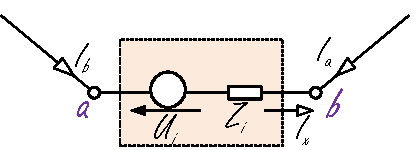
\includegraphics[width=0.7\linewidth]{Biolek_MMUN_thev_dvojpol.pdf}
          \caption[MMUN - Théveninův model dvojpólu]{Začlenění obecného lineárního dvojpólu, 
                   popsaného Théveninovým modelem do obvodu \cite[s.~78]{Biolek}}
          \label{TEO:fig_MMUN_thev_dvojpol}
        \end{figure}
        
        Původní rovnice popisující rovnováhu proudů v uzlu \emph{a} musí být na pravé straně 
        doplněna o proud $I_x$, vytékající ven z uzlu, a v uzlu \emph{b} o proud $I_x$ se záporným 
        znaménkem, protože vtéká dovnitř uzlu \emph{b}. Navíc uzlová napětí $U_a$ a $U_b$ jsou nyní 
        vázána podmínkou
        
        \begin{equation}\label{TEO:eq_MMUN_dvojpol}
          Z_iI_x + U_b = U_i + U_a, \quad\text{neboli}\quad U_i = Z_iI_x + U_b - U_a
        \end{equation}
        Všechny tyto modifikace lze zahrnout do nové soustavy rovnic MMUN:
        
        \begin{figure}[ht!]
          \centering
          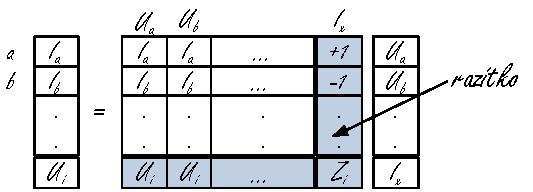
\includegraphics[width=1\linewidth]{Biolek_MMUN_razitko.pdf}
          \caption[MMUN - razítko]{ Razítko v pseudoadmitanční matici \cite[s.~79]{Biolek}}
          \label{TEO:fig_MMUN_razitko}
        \end{figure}
        
        Vektor neznámých uzlových napětí je rozšířen o další neznámou, $I_x$. Počet rovnic je 
        rovněž zvětšen o jedničku, a to o výše uvedenou podmínku mezi uzlovými napětími $U_a$ a 
        $U_b$. Přitom napětí $U_i$ je začleněno do vektoru známých budicích veličin na levé straně. 
        Modifikace rovnic 1. KZ pro uzly \emph{a} a \emph{b} je provedena zápisem $+1$ a $-1$ do 
        sloupce "$I_x$".
        
        Právě provedený zápis je návodem, jak pomocí MMUN analyzovat například obvody obsahující 
        zdroj napětí. Impedance $Z_i$ může být i nulová, pak se bude jednat o ideální zdroj napětí. 
        Při $U_i = 0$ a $I_i = 0$ lze modelovat zkrat mezi uzly a počítat proud, tekoucí tímto 
        zkratem. Toho lze využít například při analýze obvodů s proudem řízenými zdroji. 
        
        V případě, že se v obvodu nachází více prvků bez admitančního popisu, odpovídá každému z 
        nich samostatné razítko. Pseudoadmitanční matice pak nabývá na rozměrech. Metodu budeme 
        blíže konkretizovat na několika příkladech. 
  
        \subsubsection{Pasivní obvody obsahující zdroje napětí a proudu}
          Pomocí MMUN vyřešme zadání z obr. \ref{TEO:fig_MMUN02}. Je hledán proud \(I_x\) vytékající 
          ze zdroje napětí 
          %----------------------------------
          % image: TEO_fce01.tex label: \label{TEO:fig_MMUN02}
            \input{../src/TEO/img/TEO_circ02.tex}  
          %---------------------------------- 
        \subsubsection{Obvody s ideálním operačním zesilovačem ty\-pu VFA}
          Ideální OPAMP, na obr. \ref{TEO:fig_MMUN_ideal_VFA} po vložení do obvodu způsobí 
          ztotožnění uzlových napětí $U_a$ a $U_b$, a modifikaci proudových poměrů v uzlu \emph{c}.
      
          \begin{figure}[ht!]
            \centering
            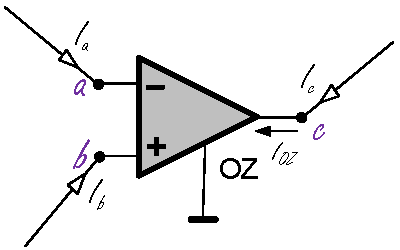
\includegraphics[width=0.6\linewidth]{MMUN_ideal_VFA.pdf}
            \caption[Ideální operační zesilovač typu VFA]{Ideální operační zesilovač typu VFA}
            \label{TEO:fig_MMUN_ideal_VFA}
          \end{figure}
          Ve spodním přídavném řádku je zapsána rovnice
          \begin{equation}\label{TEO:eq_MMUN_VFA}
              0 = 1\cdot U_a - 1\cdot U_b
          \end{equation}
          Výsledek řešení se nezmění, jestliže obě strany této rovnice vynásobíme libovolným 
          nenulovým číslem. Ve spodním řádku tedy může být namísto $[1,-1]$ například $[15,-15]$.
          \begin{figure}[ht!]
            \centering
            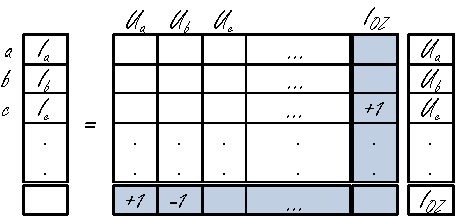
\includegraphics[width=\linewidth]{MMUN_ideal_VFA_matice.pdf}
            \caption[MMUN - pro ideální OPAMP]{MMUN - pro ideální OPAMP typu VFA}
            \label{TEO:fig_MMUN_VFA_matice}
          \end{figure}
          Je-li jeden ze vstupů OZ spojený s referenčním uzlem, neobjeví se příslušné uzlové napětí 
          v rovnicích a proto v posledním řádku bude figurovat jen jedna jednička místo uvedené 
          dvojice. 
          
          Jednička v řádku \emph{c} a sloupci $I_{OZ}$ reprezentuje připočtení proudu $I_{OZ}$ do 
          celkové bilance proudů, vytékající z uzlu \emph{c}.
        
          % --------example: Invertující zesilovač ---------------
          % \label{TEO:ex_InvOpamp01}
            % !TeX spellcheck = cs_CZ
\begin{example}\label{TEO:ex_InvOpamp01}
  Uvažujme invertující zesilovač s ideální operačním zesilovačem typu VFA s naznačenými uzly 
  tak, jak je na obr. \ref{TEO:fig_MMUN_inv_opamp}. Napište rovnice MMUN.
  
   {\centering
    \captionsetup{type=figure}
    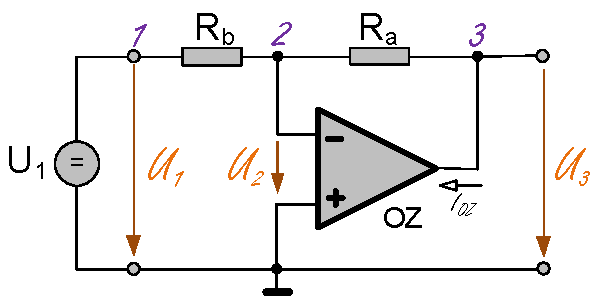
\includegraphics[width=0.7\linewidth]{MMUN_inv_OPAMP.pdf}
    \captionof{figure}{Invertující zesilovač}
    \label{TEO:fig_MMUN_inv_opamp}
    \par}
  
  Rovnice MMUN budou v maticovém zápisu vypadat takto:

    % using \usepackage{array} and command \newcolumntype{C}[1]{>{\centering}m{#1}}!
   {\centering
    \begin{tabular}{|C{0.6cm}|C{1.2cm}|C{0.6cm}|C{0.45cm}|C{0.45cm}|C{.3cm}|c|C{.33cm}|c|}
        \multicolumn{1}{c}{$U_1$}    & \multicolumn{1}{c}{$U_2$}    & \multicolumn{1}{c}{$U_3$}  & 
        \multicolumn{1}{c}{$I_1$}    & \multicolumn{1}{c}{$I_{OZ}$} & \multicolumn{1}{c}{ }      &  
        \multicolumn{1}{c}{x}        & \multicolumn{1}{c}{ }        & \multicolumn{1}{c}{b}       \\
      \cline{1-5}\cline{7-7} \cline{9-9}
      $G_b$  & $-G_b$    &  & -1  &  & \multirow{5}{*}{$\ast$} & $U_1$ & \multirow{5}{*}{=}     & \\
      \cline{1-5} \cline{7-7} \cline{9-9}
      $-G_b$ & $G_a+G_b$ & $-G_a$ &  &   & & $U_2$      &      &                                  \\
      \cline{1-5} \cline{7-7} \cline{9-9}
             & $-G_a$    & $G_a$  &  & 1 & & $U_3$      &      &                                  \\
      \cline{1-5} \cline{7-7} \cline{9-9}
         1   &           &        &  &   & & $I_1$      &      &    $U_{IN}$                      \\
      \cline{1-5} \cline{7-7} \cline{9-9}
             &     1     &        &  &   & & $I_{OZ}$   &      &                                  \\
      \cline{1-5} \cline{7-7} \cline{9-9}
    \end{tabular}
    \par}
  \vspace{1em}
  Předposlední rovnice říká, že uzlové napětí $U_1$ je rovno napětí signálového zdroje $U_{IN}$. 
  Jednička v posledním řádku reprezentuje jednoduchou rovnici $U_2 = 0$. Ačkoliv je obvod poměrně 
  jednoduchý, je pro ruční řešení neefektivní, neboť jsme získali soustavu o 5 rovnic a 5 neznámých.
\end{example}  
          %-------------------------------------------------------

          % --------example: Neinvertující zesilovač -------------
          % \label{TEO:ex_NeinvOpamp01}
            % !TeX spellcheck = cs_CZ
\begin{example}\label{TEO:ex_NeinvOpamp01} 
  Uvažujme neinvertující zesilovač s ideální operačním zesilovačem typu VFA s naznačenými uzly tak, 
  jak je na obr. \ref{TEO:fig_MMUN_neinv_opamp}. Napište rovnice MMUN.

   {\centering
    \captionsetup{type=figure}
    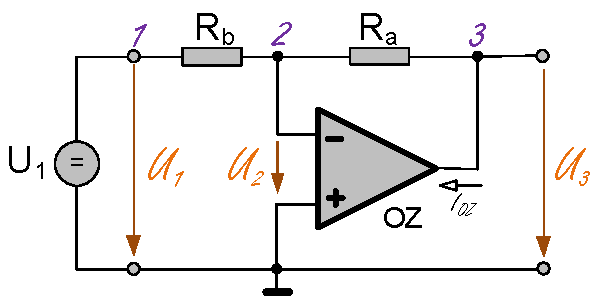
\includegraphics[width=0.7\linewidth]{MMUN_inv_OPAMP.pdf}
    \captionof{figure}{Neinvertující zesilovač}
    \label{TEO:fig_MMUN_neinv_opamp}
    \par}
   % using \usepackage{array} and command \newcolumntype{C}[1]{>{\centering}m{#1}}!
  {\centering
   \begin{tabular}{|C{0.45cm}|C{1.2cm}|C{0.6cm}|C{0.45cm}|C{0.45cm}|C{0.2cm}|c|C{.3cm}|c|}
      \multicolumn{1}{c}{$U_1$} & \multicolumn{1}{c}{$U_2$}   & \multicolumn{1}{c}{$U_3$} & 
      \multicolumn{1}{c}{$I_1$} & \multicolumn{1}{c}{$I_{OZ}$}& \multicolumn{1}{c}{ }     & 
      \multicolumn{1}{c}{x}     & \multicolumn{1}{c}{ }       & \multicolumn{1}{c}{b}     \\ 
      \cline{1-5} \cline{7-7} \cline{9-9}
           &   &   &  -1  &  & \multirow{5}{*}{$\ast$} & $U_1$ & \multirow{5}{*}{=}  &   \\
      \cline{1-5} \cline{7-7} \cline{9-9}
           & $G_a+G_b$ & $-G_a$ &      &   & & $U_2$     &   &                           \\
      \cline{1-5} \cline{7-7} \cline{9-9}
           & $-G_a$    & $G_a$ &       & 1 & & $U_3$     &   &                           \\
      \cline{1-5} \cline{7-7} \cline{9-9}
         1 &           &       &       &   & & $I_1$     &   & $U_{IN}$                  \\
      \cline{1-5} \cline{7-7} \cline{9-9}
           &     1     &       &       &   & & $I_{OZ}$  &   & $U_{IN}$                  \\
      \cline{1-5} \cline{7-7} \cline{9-9}
   \end{tabular}
   \par}
   \vspace{1em}
\end{example}  
          %-------------------------------------------------------
          \newpage
          % --------example: Diferenciální zesilovač -------------
          % \label{TEO:ex_DifOpamp01}
            % !TeX spellcheck = cs_CZ
\begin{example}\label{TEO:ex_DifOpamp01} 
  Uvažujme diferenciální zesilovač s ideální operačním zesilovačem typu VFA s naznačenými 
  uzly tak, jak je na obr. \ref{TEO:fig_MMUN_diff_opamp}. Napište rovnice MMUN.

   {\centering
    \captionsetup{type=figure}
    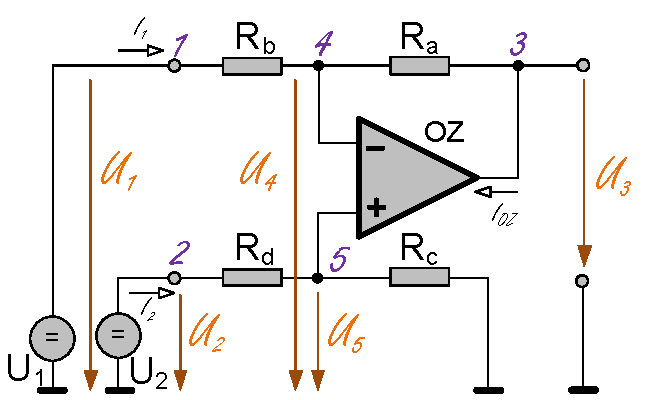
\includegraphics[width=0.7\linewidth]{MMUN_diff_OPAMP.pdf}
    \captionof{figure}{ Diferenciální zesilovač}
    \label{TEO:fig_MMUN_diff_opamp}
    \par}
%  \newpage
%  \begin{widetext}
    % using \usepackage{array} and command \newcolumntype{C}[1]{>{\centering}m{#1}}!
    {\centering
    \begin{tabular}{|C{0.6cm}|C{0.6cm}|C{0.6cm}|C{1.2cm}|C{0.6cm}|C{0.45cm}|C{0.45cm}|C{0.45cm}|}
        \multicolumn{1}{c}{$U_1$}  & \multicolumn{1}{c}{$U_2$}   & \multicolumn{1}{c}{$U_3$}  & 
        \multicolumn{1}{c}{$U_4$}  & \multicolumn{1}{c}{$U_5$}   & \multicolumn{1}{c}{$I_1$}  & 
        \multicolumn{1}{c}{$I_2$}  & \multicolumn{1}{c}{$I_{OZ}$}                      \\
        \hline
        $G_b$  &        &        & $-G_b$    &         & \(-1\) &        &             \\
        \hline
               & $G_d$  &        &           & $-G_d$  &        & \(-1\) &             \\
        \hline
               &        &  $G_a$ & $-G_a$    &         &        &        &             \\
        \hline 
        $-G_b$ &        & $-G_a$ & $G_a+G_b$ &         &        &        &             \\
        \hline
               & $-G_d$ &        & $G_c+G_d$ &         &        &        &             \\
        \hline
               &        &        &  \(-1\)   &  \(1\)  &        &        &             \\
        \hline
         1     &        &        &           &         &        &        &             \\
        \hline   
               & \(1\)  &        &           &         &        &        &             \\
        \hline    
    \end{tabular}
    \par}
%    \vspace*{0.5cm}
%  \end{widetext}
\end{example}  
          %-------------------------------------------------------

  \section{Analýza pomocí numerického simulátoru}
    \subsection{Analýza „DC“ neboli stejnosměrná analýza}
    \subsection{Rozšiřující typy analýz}
      \subsubsection{Citlivostní analýza („Sensitivity“)}
        Je počítána \emph{stejnosměrná citlivost} jedné nebo více veličin, vyjádřené vzorcem nebo 
        vzorci, na jednu nebo více vstupních proměnných.

          % --example: Citlivostní analýza napěťový děliče -------
          % \label{TEO:ex_CitDiveder01}
            % !TeX spellcheck = cs_CZ
\begin{example}\label{TEO:ex_CitDiveder01}
  V elektronických soustavách se největších přesností dosahuje u rezistorů, kde je standardně 
  zaručována chyba menší než 1\%, u přesných 0.1\% a u velmi přesných 0.01\%.

   {\centering
    \captionsetup{type=figure}
    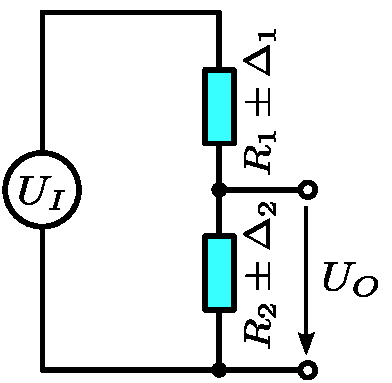
\includegraphics[width=0.4\linewidth]{voltage_divider.pdf}
    \captionof{figure}{ }
    \label{TEO:fig_voltage_divider}
    \par}

  Bude nás zajímat jaký vliv má tolerance rezistorů na výsledný poměr výstupního ku vstupnímu 
  napětí a také, zda-li při různě zvoleném poměru těchto rezistorů se bude měnit velikost chyby, 
  ačkoliv budou mít stejnou přesnost. Intuitivně předpokládáme, že  nejnepříznivější situace  
  nastane, když hodnoty použitých rezistorů padnou na opačné strany tolerančních pásem, jenž 
  reprezentuje $\Delta_1$ a $\Delta_2$ tj. $R_2 - \Delta_2R_2$ a $R_1 + \Delta_1R_1$ nebo $R_2 + 
  \Delta_2R_2$ a $R_1 - \Delta_1R_1$. V obou případech bude chyba stejná, proto si vybereme 
  například první případ a zapíšeme (rov. \ref{TEO:eq_divider_1}).
  \begin{equation}\label{TEO:eq_divider_1}
    \frac{U_o}{U_i} = \frac{R_2-\Delta_2 R_2}{R_1+\Delta_1 R_1+R_2-\Delta_2 R_2}
  \end{equation}
  a po úpravě
  \begin{equation*}
     \frac{U_o}{U_i} = \frac{(1-\Delta_2) R_2}{(1+\Delta_1) R_1+(1-\Delta_2) R_2}
  \end{equation*}
  Polynom ve jmenovateli rozvineme do následující podoby
  \begin{align*}
     [(1+\Delta_1) &+ (1-\Delta_2)](R_1+R_2)                \\
                   &= (1+\Delta_1)R_1 + (1-\Delta_2)R_2     \\
                   &+ (1+\Delta_1)R_2 + (1-\Delta_2)R_1     \\
   (1+\Delta_1)R_1 &+ (1-\Delta_2)R_2                       \\
                   &= [(1+\Delta_1)+(1-\Delta_2)](R_1+R_2)  \\
                   &- (1+\Delta_1)R_2 - (1-\Delta_2)R_1 
  \end{align*}
  a získáme %Further simplification of the denominator yields
  {\footnotesize
  \begin{equation*}
      \dfrac{U_o}{U_i}\ =
        \dfrac{(1-\Delta_2) R_2}{[(1+\Delta_1) + (1-\Delta_2)](R_1+R_2) - 
        [(1+\Delta_1) R_2\ +\ (1-\Delta_2) R_1] }
  \end{equation*}
  } %
  Nyní vydělíme jmenovatel i čitatel $(R_1 + R_2)$ a dostaneme 
  % Next divide both numerator and denominator by R1 + R2
  \begin{equation*}\label{TEO:eq_divider_2}
    \frac{U_o}{U_i}\ =\dfrac{\dfrac{(1-\Delta_2) R_2}{R_1+R2}}{[(1+\Delta_1)+(1-\Delta_2)] - 
    \dfrac{[(1+\Delta_1) R_2\ +\ (1-\Delta_2) R_1]}{R_1+R_2} }
  \end{equation*}
  Standardně rezistory volíme se stejnou tolerancí, tedy $\Delta_1 = \Delta_2 = \Delta$ a získáme 
  výslednou rovnici pro poměr $\frac{U_o}{U_i}$ 
  % Based on the assumption that both $\Delta1 = \Delta2 = \Delta$ then it should be possible to  
  % further simplify the expression for Vo/Vi:
  \begin{equation}
     \dfrac{U_o}{U_i} = \dfrac{\dfrac{(1-\Delta) R_2}{R_1+R_2}}{[(1+\Delta)+(1-\Delta)] - 
     \dfrac{[(1+\Delta)R_2 + (1-\Delta) R_1]}{R_1+R_2} }
  \end{equation}

  Řekněme například, že pro návrh děliče máme k dispozici rezistory s tolerancí 1\% a vstupní 
  napětí je 1 V. Obvod, ve kterém je dělič použit, umožňuje volit různé poměry, ale jejich součet 
  je konstantní. Na otázku jaký poměr zvolit, abychom při dané toleranci rezistorů dostali 
  výstupní napětí s největší přesností odpovídá následující tabulka.
  \vspace{1em}
  
  {\centering
   \setlength{\tabcolsep}{5pt}
   \begin{tabular}{|c|c|c|c|}
      \hline
        $R_1$                 & $1 k\Omega$  & $10 k\Omega$     & $19 k\Omega$   \\
      \hline
        $R_2$                 & $19 k\Omega$ & $10 k\Omega$     & $1 k\Omega$    \\
      \hline
        $U_{out}$             & 0,950        & 0,500            & 0,050          \\
      \hline
        $U_{out}^*$           & 0,949        & 0,495            & 0,049          \\
      \hline
        $\varepsilon_r [\%]$  & 0,101        & 1,000            & 1,883          \\
      \hline
   \end{tabular}
  \par}
  \vspace{1em}

  % Let's compare this answer to the formula I gave in a previous post using differentials. The  
  % relevant differential is
  % \begin{equation}\label{TEO:eq_divider_8}
  %   dV_0 = ( \frac{V}{R_1+R_2} - \alpha ) dR_1 - \alpha dR_2 + \frac{R_1}{R_1+R_2} dV
  % \end{equation}
  % where
  % \begin{equation}\label{TEO:eq_divider_9}
  %   \alpha = \frac{R_1 V}{(R_1+R_2)^2}
  % \end{equation}
\end{example}  
    
          %-------------------------------------------------------
} % \tikzset

%---------------------------------------------------------------------------------------------------
\printbibliography[title={Seznam literatury}, heading=subbibliography]
\addcontentsline{toc}{section}{Seznam literatury}